\section{Antennes, rayonnement, bilan de liaison}
Une antenne assure la conversion d'une onde électromagnétique \emph{guidée} en
une onde électromagnétique \emph{rayonnée} et inversement. Everything upstream
of it --- the generator, the line, the matching network --- has been engineered
so that the power arrives at the terminals of the antenne; une antenne à
l'émission doit répartir dans l'espace toute la puissance tirée du générateur,
en respectant une loi d'éclairement et une orientation des champs donnée. Three
quantities describe it completely enough to read a datasheet. On définit ainsi
trois caractéristiques essentielles pour l'antenne à l'émission :
l'\textbf{impédance d'entrée} (\textit{input impedance}) que présente l'antenne
au générateur et qui conditionne l'adaptation en puissance indispensable pour
extraire du générateur toute la puissance disponible ; le \textbf{diagramme de
rayonnement} (\textit{radiation pattern}), qui définit la répartition spatiale
de la puissance rayonnée ; la \textbf{polarisation}, qui spécifie l'orientation
du champ rayonné et son évolution en fonction du temps. The chapter closes with
the \emph{bilan de liaison}, which is the one calculation in this part the
course insists must be manipulated fluently.

\subsection{Le point sur les unités}

\begin{definition}[Décibel]
  Par définition, le \textbf{décibel} (dB) permet de quantifier un
  \emph{rapport de puissances} en échelle logarithmique,
  \[ G_{\mathrm{dB}} = 10 \log \frac{P_2}{P_1}. \]
  Il est utilisé pour exprimer le gain d'un amplificateur, l'atténuation d'un
  milieu, le gain d'une antenne --- of anything dimensionless.
\end{definition}

\begin{example}[Amplifier]
  An amplifier takes $P_1 = 2$~mW to $P_2 = 1$~W. Gain de l'amplificateur :
  $G = P_2/P_1 = 500$, sans unité ; gain de l'amplificateur en dB :
  $G_{\mathrm{dB}} = 10 \log 500 = 27$~dB.
\end{example}

\begin{definition}[dBm et dBW]
  Une puissance peut être exprimée en dBW ou dBm. Dans ce cas, la puissance est
  définie par rapport à une puissance de référence $P_{\mathrm{ref}}$ :
  \[ P_{\mathrm{dBm}} = 10 \log \frac{P}{1\ \mathrm{mW}}, \qquad
     P_{\mathrm{dBW}} = 10 \log \frac{P}{1\ \mathrm{W}}. \]
  Exemples : $1$~mW, soit $0$~dBm et $-30$~dBW ; $2$~mW, soit $3$~dBm et
  $-27$~dBW ; $1$~W, soit $0$~dBW.
\end{definition}

Since a dB is a ratio and a dBm is a power, only some combinations are legal.
This is exam bookkeeping and is worth memorising as a table rather than
re-deriving each time.

\begin{center}
  \begin{tabular}{@{}ll@{}}
    \toprule
    Opération & Résultat \\
    \midrule
    dB $+$ dB, \quad dB $-$ dB & dB \\
    dBm $+$ dB & dBm \\
    dBm $-$ dB & dBm \\
    dBm $-$ dBm & dB \\
    \midrule
    dBm $+$ dBm & pas possible \\
    dB $-$ dBm & pas possible \\
    \bottomrule
  \end{tabular}
\end{center}

\subsection{D'où vient le rayonnement ?}

\begin{definition}[Antenne]
  Une \textbf{antenne} (\textit{antenna}) est un dispositif qui assure la
  conversion d'une onde électromagnétique guidée en une onde électromagnétique
  rayonnée et inversement.
\end{definition}

Une antenne est donc reliée physiquement à un dispositif de guidage des ondes.
Il peut s'agir d'un câble coaxial, d'une ligne imprimée (ligne coplanaire,
ligne microruban, \ldots) ou d'un guide d'ondes.\\

On peut montrer qu'il existe des champs électriques et magnétiques produits en
un point $M$ de l'espace libre, par des répartitions de courants et de charges
localisées dans un volume $V'$. Les mouvements accélérés des charges sur
l'antenne créent un champ électromagnétique. Ainsi, \emph{seules les sources
(densités de courant) variables dans le temps rayonnent}. Le champ
électromagnétique se propage à la vitesse de la lumière (dans l'air ou le
vide) : $c = 3 \times 10^8$~m$\cdot$s$^{-1}$.

\begin{figure}[h!]
  \centering
  \begin{tikzpicture}[>=latex,scale=1.0]
    \draw[->] (0,0) -- (0,1.9) node[left] {$z$};
    \draw[->] (0,0) -- (2.4,0) node[below] {$y$};
    \draw[->] (0,0) -- (-1.05,-0.95) node[below] {$x$};
    \draw[thick] (5.0,0.9) ellipse (1.05 and 0.78);
    \node at (5.0,-0.15) {\small $V'$ --- antenne};
    \fill (4.85,0.95) circle (1.3pt);
    \node[below] at (4.9,0.92) {\small $M'$};
    \node[right] at (6.15,1.15) {\small $\v{j}(\v{r}',t),\ \rho(\v{r}',t)$};
    \fill (5.9,3.1) circle (1.3pt);
    \node[above right] at (5.9,3.1) {\small $M$};
    \node[left] at (5.85,3.2) {\small $\v{E}(\v{r},t),\ \v{H}(\v{r},t)$};
    \draw[->] (0,0) -- (5.84,3.06) node[pos=0.62,above,sloped] {\small $\v{r}$};
    \draw[->] (0,0) -- (4.80,0.93) node[pos=0.6,below,sloped] {\small $\v{r}'$};
    \draw[->] (4.85,0.95) -- (5.86,3.06) node[pos=0.55,right] {\small $\v{r}-\v{r}'$};
  \end{tikzpicture}
\end{figure}

\begin{remark}[Retarded time]
  Le champ électromagnétique en $M$ à l'instant $t$ dépend de l'état des
  sources à l'instant \emph{antérieur}
  \[ t' = t - \frac{\|\v{r} - \v{r}'\|}{c}, \]
  which is what makes the radiated field a propagating object rather than an
  instantaneous one.
\end{remark}

Les équations de Maxwell permettent de relier le champ électromagnétique et les
courants/charges. The course writes them with $\operatorname{rot}$ and
$\operatorname{div}$:
\[
  \curl \v{E} = -\frac{\del \v{B}}{\del t}, \qquad
  \curl \v{H} = \v{j} + \frac{\del \v{D}}{\del t}, \qquad
  \div \v{D} = \rho, \qquad \div \v{B} = 0,
\]
dans le vide : $\v{B} = \mu_0 \v{H}$ et $\v{D} = \epsilon_0 \v{E}$. La
connaissance des courants sur l'antenne permet donc le calcul du champ
électromagnétique rayonné : $\{\v{j}, \rho\} \lra \{\v{E}, \v{H}\}$.

\begin{remark}[Design constraints]
  Electrical performance is only one constraint. Pour qu'une antenne présente
  de « bonnes » performances, ses dimensions sont de l'ordre de la
  demi-longueur d'onde --- pour les fréquences LTE autour de 700~MHz, la
  longueur d'onde est égale à 43~cm, so $\lambda/2 \approx 21.5$~cm, which is
  why small multiband terminal antennes are hard. Les antennes doivent être
  discrètes et petites pour des raisons esthétiques, mais parfois aussi pour
  des raisons aérodynamiques. Une antenne doit parfois, si son environnement
  l'exige, être capable de fonctionner sur une grande gamme de température
  (typiquement $-120$ à $+120\,^\circ$C sur un satellite) et/ou supporter de
  fortes puissances (kW sur un radar d'aéroport).
\end{remark}

\subsection{Impédance d'entrée de l'antenne}

L'impédance d'entrée de l'antenne est une grandeur complexe :
$Z_{\mathrm{ant}} = R_{\mathrm{ant}} + j X_{\mathrm{ant}}$. L'impédance de
sortie de l'émetteur, $50\ \Omega$, is the usual reference.

\begin{definition}[Facteur de réflexion à l'entrée de l'antenne]
  Le \textbf{facteur de réflexion} du signal à l'entrée de l'antenne est
  \[ \Gamma_{\mathrm{ant}} = \frac{Z_{\mathrm{ant}} - Z_C}{Z_{\mathrm{ant}} + Z_C}, \]
  où $Z_C$ est l'impédance caractéristique de la ligne d'accès à l'antenne
  (câble coaxial, guide d'ondes, \ldots). $\Gamma_{\mathrm{ant}}$ est une
  grandeur complexe ; c'est le rapport entre la tension réfléchie et la
  tension incidente à l'entrée de l'antenne.
\end{definition}

Lorsque $Z_{\mathrm{ant}} = Z_C$, il n'y a pas de réflexion à l'entrée de
l'antenne. C'est le cas idéal. Malheureusement, l'impédance $Z_{\mathrm{ant}}$
dépend de la fréquence ; d'autre part, les caractéristiques d'une antenne et
donc son impédance d'entrée dépendent de l'environnement. On ne peut donc
obtenir un facteur de réflexion nul sur toute la bande souhaitée quel que soit
l'environnement. Néanmoins, le travail du concepteur d'antenne consiste à le
minimiser.\\

Because $\Gamma$ is a voltage ratio, le rapport entre la puissance réfléchie et
la puissance incidente (c'est-à-dire la puissance issue du générateur si on
considère une ligne d'accès sans pertes) s'écrit
$|\Gamma_{\mathrm{ant}}|^2 = P_{\mathrm{refl}} / P_{\mathrm{gen}}$. La
puissance transmise à l'antenne est donc

\[ \boxed{P_{\mathrm{ant}} = \bigl(1 - |\Gamma_{\mathrm{ant}}|^2\bigr) P_{\mathrm{gen}}.} \]

$P_{\mathrm{ant}}$ n'est \emph{pas} la puissance rayonnée : il existe d'autres
pertes au niveau de l'antenne (pertes métalliques, diélectriques, \ldots).

\begin{definition}[Efficacité de rayonnement]
  Avec $e_{\mathrm{ray}}$ l'\textbf{efficacité de rayonnement}
  (\textit{radiation efficiency}), $0 < e_{\mathrm{ray}} < 1$, la puissance
  rayonnée par l'antenne s'écrit
  \[ P_{\mathrm{ray}} = e_{\mathrm{ray}} P_{\mathrm{ant}}, \qquad
     P_{\text{dissipée}} = (1 - e_{\mathrm{ray}}) P_{\mathrm{ant}}. \]
\end{definition}

\begin{figure}[h!]
  \centering
  \begin{tikzpicture}[>=latex,scale=1.0]
    \draw[thick] (0,0) rectangle (1.7,1.1);
    \node[align=center] at (0.85,0.55) {\small générateur};
    \draw[thick] (1.7,0.75) -- (4.3,0.75);
    \draw[thick] (1.7,0.35) -- (4.3,0.35);
    \node[align=center] at (3.0,-0.15) {\small ligne, $Z_C$};
    \draw[thick] (4.3,0) rectangle (6.0,1.1);
    \node[align=center] at (5.15,0.55) {\small antenne};
    \draw[->,thick] (2.0,1.45) -- (3.2,1.45) node[midway,above] {\small $P_{\mathrm{gen}}$};
    \draw[<-,thick] (3.6,1.45) -- (4.2,1.45);
    \node[above] at (3.9,1.5) {\small $|\Gamma_{\mathrm{ant}}|^2 P_{\mathrm{gen}}$};
    \draw[->,thick] (6.0,0.55) -- (7.2,0.55) node[right] {\small $P_{\mathrm{ray}} = e_{\mathrm{ray}} P_{\mathrm{ant}}$};
    \draw[->,thick] (5.15,0) -- (5.15,-0.85) node[below] {\small $P_{\text{dissipée}} = (1-e_{\mathrm{ray}})P_{\mathrm{ant}}$};
  \end{tikzpicture}
\end{figure}

\subsubsection{Bande passante}

Les caractéristiques d'une antenne et donc son facteur de réflexion
$\Gamma_{\mathrm{ant}}$ dépendent de la fréquence. Il est donc nécessaire
d'observer les performances d'une antenne sur la ou les bandes de fréquences
d'utilisation. En échelle logarithmique,
\[ |\Gamma_{\mathrm{ant}}|_{\mathrm{dB}} = 20 \log |\Gamma_{\mathrm{ant}}|, \]
the factor $20$ being there because le facteur de réflexion $\Gamma$ est un
rapport de tension et non de puissance.

\begin{remark}[Voltage ratio, not power ratio]
  The factor $20$ is what a voltage ratio calls for; were $\Gamma$ a ratio of
  powers, its expression in dB would carry a factor ten instead.
\end{remark}

\begin{definition}[Bande passante en adaptation]
  Il existe de nombreuses définitions de la bande passante. La plus commune est
  la \textbf{bande passante en adaptation} (\textit{matching bandwidth}), où le
  module du facteur de réflexion de l'antenne $|\Gamma_{\mathrm{ant}}|$ est
  inférieur à un certain niveau (généralement $-10$~dB).
\end{definition}

\begin{example}[Antenne de téléphonie mobile]
  For one commercial antenne, en prenant comme critère
  $|\Gamma_{\mathrm{ant}}|_{\mathrm{dB}} < -6$~dB, valeur typique pour des
  antennes de téléphone mobile, les bandes passantes mesurées sont
  $[700 - 960]$~MHz, $[1.75 - 2.3]$~GHz, $[2.56 - 2.65]$~GHz et
  $[3.1 - 4.38]$~GHz. Cette antenne couvre donc les standards GSM900/1800,
  PCS1900, UMTS2100 et LTE700/2300/2600/3400/3600.
\end{example}

\subsubsection{Rapport d'ondes stationnaires}

\begin{definition}[ROS / VSWR]
  Pour caractériser une antenne en adaptation, au lieu d'étudier
  $|\Gamma_{\mathrm{ant}}|_{\mathrm{dB}}$ dans la bande de fréquences souhaitée,
  on utilise parfois le rapport d'onde stationnaire (ROS) ou VSWR (Voltage
  Standing Wave Ratio) :
  \[ \mathrm{ROS} = \mathrm{VSWR} = \frac{1 + |\Gamma_{\mathrm{ant}}|}{1 - |\Gamma_{\mathrm{ant}}|},
     \qquad\text{equivalently}\qquad
     |\Gamma_{\mathrm{ant}}| = \frac{\mathrm{ROS} - 1}{\mathrm{ROS} + 1}. \]
  Un ROS de $2$ correspond à $|\Gamma_{\mathrm{ant}}|_{\mathrm{dB}} = -9.5$~dB.
\end{definition}

\begin{problem}[Critère d'adaptation d'une antenne]
  Vous recherchez une antenne adaptée dans la bande $3.1 - 5$~GHz. Le système
  sur lequel vous voulez l'intégrer requiert un $\mathrm{ROS} < 2$. Un
  constructeur vous propose une antenne et vous fournit la courbe du module du
  facteur de réflexion $|\Gamma|$ en fonction de la fréquence. Cette antenne
  répond-elle à vos besoins ? Supposons que votre chaîne de transmission
  requiert un $\mathrm{ROS} < 1.4$ : mêmes questions.
\end{problem}

\begin{proof}
  Convert the criterion into a level on the supplied curve. On calcule la
  valeur du module du facteur de réflexion correspondant à un
  $\mathrm{ROS} = 2$ :
  \[ |\Gamma| = \frac{2-1}{2+1} = \frac{1}{3}, \qquad
     |\Gamma|_{\mathrm{dB}} = 20 \log \tfrac{1}{3} = -9.5\ \mathrm{dB}. \]
  La bande passante de l'antenne est l'intervalle de fréquences dans lequel
  $|\Gamma|_{\mathrm{dB}} \le -9.5$~dB. On the supplied curve, la bande passante
  de l'antenne est donc $[3.1 - 5]$~GHz soit $1.9$~GHz. L'antenne répond au
  cahier des charges pour la bande passante.\\

  On suppose un $\mathrm{ROS} = 1.4$ : $|\Gamma| = 0.4/2.4 = 1/6$ et
  $|\Gamma|_{\mathrm{dB}} = -15.6$~dB. Avec le nouveau critère, la bande
  passante est de $500$~MHz comprise dans l'intervalle $[4.25 - 4.75]$~GHz, ce
  qui ne convient donc plus au cahier des charges demandé. \qed
\end{proof}

\subsection{Diagramme de rayonnement}

Le diagramme de rayonnement est une représentation graphique de la répartition
spatiale de la puissance rayonnée par l'antenne.

\subsubsection{Champ lointain et coordonnées sphériques}

\begin{definition}[Champ lointain]
  Pour tracer un diagramme de rayonnement, on s'intéresse au rayonnement en
  \textbf{champ lointain} (\textit{far field}), c'est-à-dire loin des sources
  (antenne). En général, la zone de champ lointain est située au-delà d'une
  distance, appelée \textbf{distance de Fraunhofer}
  (\textit{Fraunhofer distance}),
  \[ r > \frac{2 D^2}{\lambda}, \]
  $D$ étant la plus grande dimension de l'antenne et $\lambda$ la longueur
  d'onde.
\end{definition}

Dans la zone de champ lointain, les ondes électromagnétiques se propageant sont
des ondes \emph{sphériques}. L'amplitude des champs $\v{E}$ et $\v{H}$ varie en
$1/r$. Localement, l'onde pourra être considérée comme plane, so that the ratio
of the field magnitudes is the impédance d'onde du vide
\[ \frac{E}{H} = \eta_0 = \sqrt{\frac{\mu_0}{\epsilon_0}} = 120\pi = 377\ \Omega. \]
Les coordonnées sphériques $(r, \theta, \varphi)$ sont souvent utilisées pour
tracer le diagramme de rayonnement, $\theta$ being the angle from $Oz$ and
$\varphi$ the azimuth in $xOy$.

\subsubsection{Densité surfacique de puissance et puissance rayonnée}

La puissance d'une onde électromagnétique s'exprime par le vecteur de Poynting.
La moyenne temporelle du vecteur de Poynting en régime harmonique en $M$
s'écrit
\[ \v{\Pi}(r,\theta,\varphi) = \frac{\Re\bigl(\v{E} \wedge \v{H}^{*}\bigr)}{2}, \]
and its norm $p(r,\theta,\varphi) = \|\v{\Pi}(r,\theta,\varphi)\|$, en
W$/$m$^2$, représente la \textbf{densité de puissance surfacique} au point
$M$.

\begin{definition}[Puissance totale rayonnée]
  La \textbf{puissance totale rayonnée} (\textit{total radiated power}) est
  égale au flux du vecteur de Poynting à travers une sphère de rayon $r$
  entourant l'antenne :
  \[ P_{\mathrm{ray}} = \oint\!\!\!\!\oint_{\text{sphère}} \v{\Pi} \cdot \mathrm{d}\v{S}
     = \int_{\theta=0}^{\pi} \int_{\varphi=0}^{2\pi}
       p(r,\theta,\varphi)\, r^2 \sin\theta \,\mathrm{d}\theta\, \mathrm{d}\varphi. \]
\end{definition}

\subsubsection{Directivité et gain d'une antenne}

Pour quantifier l'aptitude d'une antenne à rayonner l'énergie dans une
direction donnée, on la compare à l'\textbf{antenne isotrope}
(\textit{isotropic antenna}), c'est-à-dire à une antenne qui rayonne toute son
énergie de manière uniforme dans tout l'espace. La densité surfacique de
puissance de l'antenne isotrope est donc
\[ p_{\mathrm{iso}}(r) = \frac{P_{\mathrm{ray}}}{4\pi r^2}. \]

\begin{definition}[Directivité et gain]
  La \textbf{directivité} (\textit{directivity}) et le \textbf{gain} d'une
  antenne sont définis par
  \[ D(\theta,\varphi) = \frac{p(r,\theta,\varphi)}{p_{\mathrm{iso}}(r)}
     = \frac{p(r,\theta,\varphi)}{P_{\mathrm{ray}}}\, 4\pi r^2,
     \qquad
     G(\theta,\varphi) = \frac{p(r,\theta,\varphi)}{P_{\mathrm{ant}}}\, 4\pi r^2
     = e_{\mathrm{ray}} D(\theta,\varphi). \]
  La directivité s'exprime généralement en dBi ($i$ : isotrope),
  $D(\theta,\varphi)_{\mathrm{dBi}} = 10 \log D(\theta,\varphi)$ ; le gain
  s'exprime plutôt en dB, ou en dBi.
\end{definition}

\begin{remark}
  The directivité is normalised by construction: la directivité d'une antenne
  \emph{ne peut} être supérieure à $1$ dans toutes les directions. Une
  directivité élevée dans une direction donnée est obtenue au détriment des
  autres directions. The distinction between $D$ and $G$ is exactly the
  efficacité de rayonnement, qui représente les pertes dans l'antenne (pertes
  métalliques et diélectriques).
\end{remark}

\subsubsection{Les différentes représentations graphiques du diagramme de rayonnement}

Le \emph{diagramme en 3D}, plotting $D$ or $G$ in dB over the sphere, apporte
une information essentiellement qualitative sur les directions de rayonnement
ou d'absence de rayonnement. Afin d'obtenir une information plus quantitative,
on réalise des \textbf{plans de coupe} (\textit{cutting plane}) à partir du
diagramme 3D, for instance $\varphi = 0$ ; le diagramme dans un plan peut être
tracé en coordonnées polaires ou cartésiennes.

\begin{figure}[h!]
  \centering
  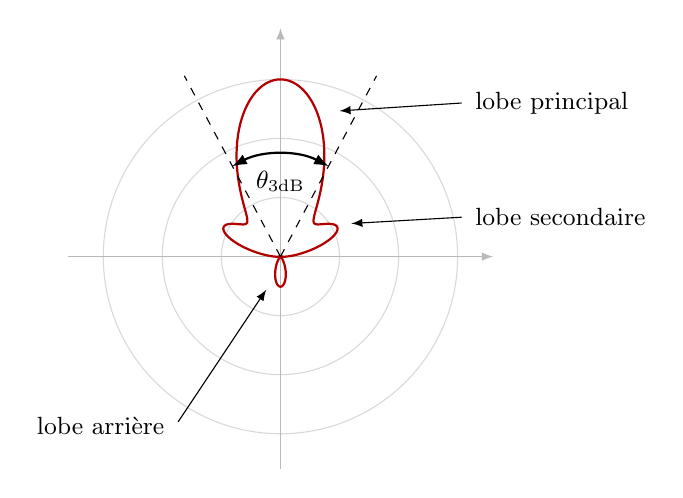
\begin{tikzpicture}[>=latex,scale=1.0]
    \foreach \rr in {0.75,1.5,2.25} { \draw[gray!30] (0,0) circle (\rr); }
    \draw[gray!55,->] (-2.7,0) -- (2.7,0);
    \draw[gray!55,->] (0,-2.7) -- (0,2.9);
    \draw[thick,red!70!black,samples=361,domain=-180:180,smooth]
      plot ({\x+90}:{2.25*(exp(-((\x)/34)^2) + 0.33*exp(-((\x-64)/17)^2)
        + 0.33*exp(-((\x+64)/17)^2) + 0.17*exp(-((\x-180)/24)^2)
        + 0.17*exp(-((\x+180)/24)^2))});
    \draw[dashed] (0,0) -- (62:2.6);
    \draw[dashed] (0,0) -- (118:2.6);
    \draw[<->,thick] (62:1.3) arc (62:118:1.3);
    \node at (0,0.95) {\small $\theta_{3\mathrm{dB}}$};
    \node[align=center,right] at (2.35,1.95) {\small lobe principal};
    \draw[->] (2.3,1.95) -- (0.75,1.85);
    \node[align=center,right] at (2.35,0.5) {\small lobe secondaire};
    \draw[->] (2.3,0.5) -- (0.9,0.42);
    \node[align=center,left] at (-1.35,-2.15) {\small lobe arrière};
    \draw[->] (-1.3,-2.1) -- (-0.18,-0.42);
  \end{tikzpicture}
\end{figure}

Le \textbf{lobe principal} (\textit{main lobe}) est défini entre les deux
minima de chaque côté du maximum. Des maxima secondaires apparaissent de chaque
côté. Ils constituent les \textbf{lobes secondaires} (\textit{side lobe}), the
one opposite the main beam being the \textbf{lobe arrière}
(\textit{back lobe}).

\begin{definition}[Ouverture à $-3$~dB]
  L'\textbf{ouverture à $-3$~dB} (\textit{beamwidth}), notée
  $\theta_{3\mathrm{dB}}$, est la plage angulaire sur laquelle
  $G_{\mathrm{dB}} \ge G_{\max,\mathrm{dB}} - 3$~dB. On parle également
  d'ouverture à mi-puissance (HPBW).
\end{definition}

Un diagramme 2D (représentation polaire ou cartésienne) peut également être
\emph{normalisé} par rapport à la directivité (ou gain) maximale. Dans ce cas,
le maximum de la courbe est $0$~dB. On perd alors l'information du gain
maximal $G_{\max}$, mais la lecture des niveaux relatifs entre les lobes est
directe.

\begin{example}[Reading a diagramme de rayonnement]
  A simulated diagramme de rayonnement at $2.18$~GHz, cut at
  $\varphi = 0^\circ$, reports: lobe principal magnitude $5.9$~dBi, lobe
  principal direction $65.0^\circ$, angular width ($3$~dB) $145.8^\circ$, lobe
  secondaire level $-11.2$~dB relative to the peak. The simulator readout
  gives the bare number ``Frequency $= 2.18$'' with no unit; GHz is inferred
  from the context.
\end{example}

\subsection{Polarisation}

La polarisation du champ électromagnétique rayonné par une antenne est donnée
par la \emph{direction du champ électrique}. On considère une propagation
suivant $Oz$ ; de façon générale, le champ électrique s'écrit
\[ \v{E} = \v{E}_x + \v{E}_y, \qquad
   \v{E}_x = E_{0x}\, e^{j(\omega t - kz)}\, \unitv{e}_x, \qquad
   \v{E}_y = E_{0y}\, e^{j(\omega t - kz + \varphi)}\, \unitv{e}_y. \]
The three cases are distinguished entirely by the déphasage $\varphi$ between
the components and by the two amplitudes.

\begin{definition}[Polarisation rectiligne]
  \textbf{Polarisation rectiligne} (\textit{rectilinear polarisation}) ou
  linéaire : la direction du vecteur $\v{E}$ ne varie pas lors de la
  propagation. Au cours du temps, l'extrémité du vecteur décrit une droite dans
  un plan orthogonal à l'axe de propagation. Le déphasage entre les composantes
  est $\varphi = 0$ ou $\varphi = \pi$.
\end{definition}

\begin{definition}[Polarisation circulaire]
  \textbf{Polarisation circulaire} (\textit{circular polarisation}) : la
  direction du vecteur $\v{E}$ varie lors de la propagation. Au cours du temps,
  l'extrémité du vecteur décrit un cercle dans un plan orthogonal à l'axe de
  propagation. This requires
  \[ \varphi = \pm \frac{\pi}{2} \qquad\text{and}\qquad E_{0x} = E_{0y}. \]
  Si $\varphi = -\pi/2$ : \textbf{polarisation circulaire droite}
  (\textit{right-handed}) ; si $\varphi = +\pi/2$ : \textbf{polarisation
  circulaire gauche} (\textit{left-handed}).
\end{definition}

\begin{remark}[The handedness convention]
  Par convention, la polarisation est dite « droite » pour l'observateur qui
  voit \emph{s'éloigner} l'onde, le champ électrique tourne alors dans le sens
  des aiguilles d'une montre (anti-trigonométrique). Elle est dite « gauche »
  dans le cas contraire. The convention is stated with respect to the
  observer, so it must be quoted with its reference or it is meaningless.
\end{remark}

\begin{definition}[Polarisation elliptique]
  \textbf{Polarisation elliptique} (\textit{elliptical polarisation}) : au
  cours du temps, l'extrémité du vecteur $\v{E}$ décrit une ellipse dans un
  plan orthogonal à l'axe de propagation. Le déphasage entre les composantes
  $\varphi$ est quelconque. Polarisation rectiligne and polarisation circulaire
  are its two degenerate cases.
\end{definition}

\begin{definition}[Polarisation croisée (\textit{cross-polarisation})]
  L'antenne peut présenter des défauts et rayonner un champ électrique avec une
  polarisation dégradée. On appelle \textbf{composante principale ou copolaire}
  (\textit{co-polar component}) la composante de champ désirée et
  \textbf{composante croisée} (\textit{cross-polar component}) celle non
  voulue. La composante croisée doit donc être la plus faible possible.
\end{definition}

\begin{example}[Antenne quasi-Yagi]
  For the quasi-Yagi antenne, la polarisation souhaitée est une polarisation
  linéaire suivant la direction des brins, $Ox$, with propagation along $Oz$ ;
  le champ $\v{E}$ est transverse (plan $xOy$). The component along $Ox$ is the
  composante principale ou copolaire, the residual component along $Oy$ is the
  composante croisée.
\end{example}

\subsection{Quelques antennes usuelles}

\subsubsection{Antennes filaires}

Les \textbf{antennes filaires} (\textit{wire antennas}) sont composées d'un ou
plusieurs conducteurs linéaires de diamètre faible. Le diagramme de rayonnement
est calculé à partir de la densité de courant sur l'antenne. Les antennes de
base sont les dipôles, les monopôles, les boucles ; des structures plus
évoluées sont les hélices, les antennes Yagi, les log-périodiques.

\paragraph{Antenne dipôle} Un dipôle est une antenne filaire composée de deux
brins conducteurs et alimentée au centre. La forme la plus courante est le
\textbf{dipôle demi-onde} (\textit{half-wave dipole}) ; la longueur de chaque
brin est dans ce cas égale à $\lambda/4$. La répartition de l'intensité du
courant le long du dipôle demi-onde est
\[ i(z,t) = I_0 \cos\!\left(\frac{2\pi z}{\lambda}\right) e^{j \omega t}, \]
maximal at the feed point and vanishing at the two ends. La polarisation d'un
dipôle est linéaire et le champ électrique $\v{E}$ est parallèle au dipôle.
L'impédance d'entrée du dipôle demi-onde est
\[ Z_{\mathrm{in}} = 73 + j\,42\ \Omega. \]

À grande distance (champ lointain), le champ rayonné peut être calculé :
\[ E_\theta(r,\theta) = -j \frac{60}{r} I_0
     \frac{\cos\left(\frac{\pi}{2}\cos\theta\right)}{\sin\theta}\,
     e^{j(\omega t - kr)},
   \qquad H_\varphi(r,\theta) = \frac{E_\theta(r,\theta)}{Z_0}, \]
avec $Z_0 = 377\ \Omega$ l'impédance d'onde du vide. On peut noter que les
champs sont transverses et que leur amplitude décroît en $1/r$ ; et que les
champs ne dépendent pas de l'angle $\varphi$, ce qui est cohérent avec la
symétrie cylindrique de l'antenne.

\begin{prop}[Directivité du dipôle demi-onde]
  \[ D(\theta) = 1.64 \left(\frac{\cos\left(\frac{\pi}{2}\cos\theta\right)}{\sin\theta}\right)^{2}. \]
  Pour $\theta = \pi/2$, la directivité est maximale :
  $D_{\max} = 1.64$ soit $2.15$~dBi. Pour $\theta = 0$ ou $\pi$, la directivité
  est nulle : un dipôle ne rayonne pas suivant son axe.
\end{prop}

\begin{remark}
  La directivité étant maximale et identique sur un plan (ici le plan $xOy$),
  le rayonnement est dit \textbf{omnidirectionnel} (\textit{omnidirectional})
  --- à ne pas confondre avec \emph{isotrope}. Omnidirectionnel means uniform
  in one plane; isotrope would mean uniform over the whole sphere, and no real
  antenne is isotrope.
\end{remark}

\begin{figure}[h!]
  \centering
  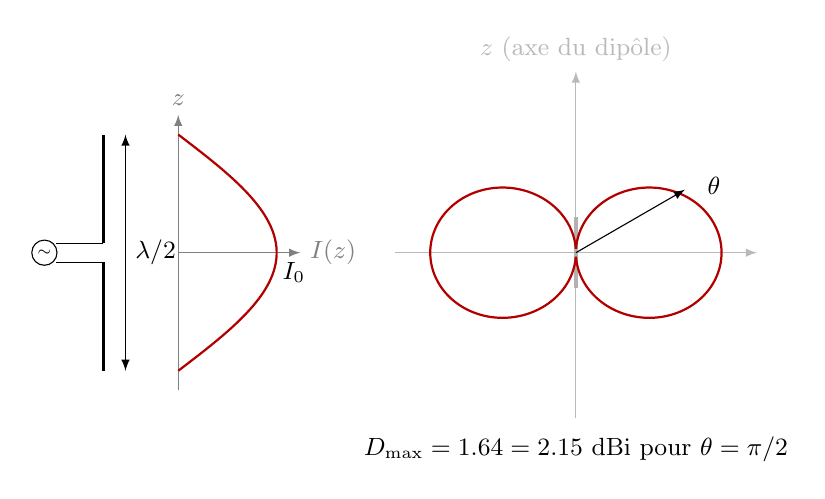
\begin{tikzpicture}[>=latex,scale=1.0]
    % left panel: current distribution
    \begin{scope}[xshift=0cm]
      \draw[very thick] (0,0.12) -- (0,1.5);
      \draw[very thick] (0,-0.12) -- (0,-1.5);
      \draw (0,0.12) -- (-0.45,0.12);
      \draw (0,-0.12) -- (-0.45,-0.12);
      \draw (-0.45,0.12) -- (-0.6,0.12);
      \draw (-0.45,-0.12) -- (-0.6,-0.12);
      \draw (-0.75,0) circle (0.16);
      \node at (-0.75,0) {\tiny $\sim$};
      \draw[<->] (0.28,-1.5) -- (0.28,1.5) node[midway,right] {\small $\lambda/2$};
      \draw[->,gray] (0.95,-1.75) -- (0.95,1.75) node[above] {\small $z$};
      \draw[->,gray] (0.95,0) -- (2.5,0) node[right] {\small $I(z)$};
      \draw[thick,red!70!black,samples=60,domain=-1:1,smooth]
        plot ({0.95+1.25*cos(90*\x)},{1.5*\x});
      \node[below right] at (2.15,0) {\small $I_0$};
    \end{scope}
    % right panel: pattern
    \begin{scope}[xshift=6.0cm]
      \draw[gray!55,->] (0,-2.1) -- (0,2.3) node[above] {\small $z$ (axe du dipôle)};
      \draw[gray!55,->] (-2.3,0) -- (2.3,0);
      \draw[very thick,gray!60] (0,-0.45) -- (0,0.45);
      \draw[thick,red!70!black,samples=180,domain=2:178,smooth]
        plot ({90-\x}:{1.85*abs(cos(90*cos(\x))/sin(\x))});
      \draw[thick,red!70!black,samples=180,domain=2:178,smooth]
        plot ({90+\x}:{1.85*abs(cos(90*cos(\x))/sin(\x))});
      \node[right] at (1.55,0.85) {\small $\theta$};
      \draw[->] (0,0) -- (30:1.6);
      \node at (0,-2.5) {\small $D_{\max} = 1.64 = 2.15$ dBi pour $\theta = \pi/2$};
    \end{scope}
  \end{tikzpicture}
\end{figure}

\paragraph{Antenne monopôle quart d'onde} Une antenne \textbf{monopôle quart
d'onde} (\textit{quarter-wave monopole}) est constituée d'un seul brin de
l'antenne dipôle demi-onde, de longueur $\lambda/4$ et situé au-dessus d'un
plan conducteur qui joue le rôle de réflecteur. Si le plan réflecteur est un
conducteur électrique parfait de dimensions infinies, on peut appliquer le
\emph{principe des images} : le rayonnement dans le demi-espace supérieur est
identique à celui d'un dipôle demi-onde. On note néanmoins que la directivité
augmente de $3$~dB compte-tenu que toute la puissance se trouve uniquement dans
le demi-espace supérieur. Lorsque le plan réflecteur est de dimensions finies
(say a disque de rayon $2\lambda$), la forme du diagramme de rayonnement change
mais la symétrie cylindrique est conservée.

\begin{figure}[h!]
  \centering
  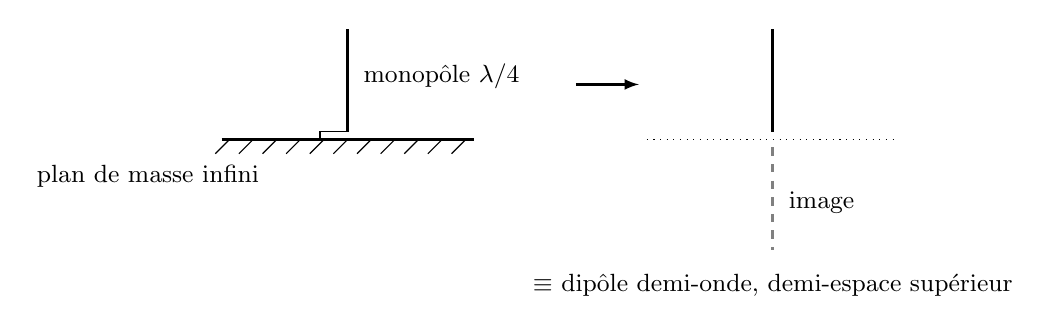
\begin{tikzpicture}[>=latex,scale=1.0]
    \draw[very thick] (0,0.1) -- (0,1.4);
    \node[right] at (0.08,0.8) {\small monopôle $\lambda/4$};
    \draw[thick] (-1.6,0) -- (1.6,0);
    \foreach \x in {-1.5,-1.2,...,1.55} { \draw (\x,0) -- (\x-0.18,-0.18); }
    \node[below left] at (-1.0,-0.2) {\small plan de masse infini};
    \draw (0,0.1) -- (-0.35,0.1) -- (-0.35,0.0);
    \draw[->,thick] (2.9,0.7) -- (3.7,0.7);
    \begin{scope}[xshift=5.4cm]
      \draw[very thick] (0,0.1) -- (0,1.4);
      \draw[very thick,dashed,gray] (0,-0.1) -- (0,-1.4);
      \draw[dotted] (-1.6,0) -- (1.6,0);
      \node[right] at (0.08,-0.8) {\small image};
      \node at (0,-1.85) {\small $\equiv$ dipôle demi-onde, demi-espace supérieur};
    \end{scope}
  \end{tikzpicture}
\end{figure}

\paragraph{Applications des antennes demi-ondes et quart d'ondes} Compte-tenu
de leur rayonnement omnidirectionnel, les antennes demi-ondes et quart d'ondes
sont utilisées pour la diffusion (TNT, radio) et pour les communications
point-multipoints (WiFi, etc.).

\paragraph{Antenne dipôle replié} L'antenne \textbf{dipôle replié}
(\textit{folded dipole}) est constituée de deux dipôles demi-ondes connectés
entre eux aux extrémités et espacés d'une distance très inférieure à la
longueur d'onde. Le dipôle replié a les mêmes caractéristiques que le dipôle
mais une impédance d'entrée plus élevée et une bande passante supérieure ; the
exact increase depends on the diameter of the dipôles and on their spacing. A
VHF example is the DigiTek antenne around $200$~MHz.

\paragraph{Effet d'éléments parasites} Si on place un dipôle \emph{non
alimenté} proche du dipôle initial, on alimente celui-ci par couplage. En
choisissant des tailles légèrement différentes de ces parasites, on peut créer
des comportements \textbf{réflecteur} (\textit{reflector}) ou
\textbf{directeur} (\textit{director}). For example, with a $30$~mm dipôle
actif and a $15$~mm spacing, a $26$~mm parasite acts as a directeur (shorter
than the driven element, beam pulled towards it), a $34$~mm parasite as a
réflecteur (longer, beam pushed away from it). It is thus the $34$~mm element
that gives the comportement réflecteur, and its diagramme de rayonnement is
that of a réflecteur.

\paragraph{Antenne Yagi} L'antenne \textbf{Yagi} (ou Yagi-Uda) comporte un
élément actif (usually a dipôle replié), un réflecteur et un ensemble de
directeurs, dipôles passifs colinéaires. L'objectif est d'obtenir une antenne
large bande et directive. Elle est couramment employée pour la réception de la
télévision.

\begin{center}
  \begin{tabular}{@{}ll@{}}
    \toprule
    Impédance d'entrée & $75\ \Omega$ (grand public) \\
    Gain & $4$~dB pour un directeur, $20$~dB pour 20 directeurs \\
    $\theta_{3\mathrm{dB}}$ & de $60^\circ$ (faible gain) à $25^\circ$ (grand gain) \\
    Rapport avant/arrière & en général $> 25$~dB \\
    \bottomrule
  \end{tabular}
\end{center}

Le \textbf{rapport avant/arrière} (\textit{front-to-back ratio}, AV/AR) est la
différence de niveau de puissance captée par le dipôle pour un signal de même
intensité, en provenance de l'avant et de l'arrière de l'antenne. Une antenne
Yagi commerciale pour la réception TNT, $[470 - 790]$~MHz, quotes
$\theta_{3\mathrm{dB}} = 40^\circ$, $G_{\max} = 15$~dB and AV/AR $= 23$~dB ;
on remarquera que le réflecteur est constitué d'une grille repliée afin de
maximiser l'effet réflecteur et augmenter davantage la directivité.

\subsubsection{Antenne à ouverture rayonnante}

Une \textbf{ouverture rayonnante} (\textit{radiating aperture}) plane est une
ouverture de surface quelconque dans un plan conducteur, illuminé par une onde
incidente. Selon le principe de Huygens, le champ rayonné en un point $P$ est
la superposition du rayonnement de sources secondaires réparties sur
l'ouverture.

\begin{prop}[Directivité maximale d'une ouverture rayonnante]
  En première approximation, il est possible à partir des champs calculés en
  $P$, situé très loin de l'ouverture, d'établir l'expression de la directivité
  maximale de l'ouverture rayonnante :
  \[ D_{\max} = \frac{4 \pi A}{\lambda^2}, \]
  $A$ étant la surface de l'ouverture.
\end{prop}

\paragraph{Antenne cornet} L'\textbf{antenne cornet} (\textit{horn antenna})
est une antenne métallique constituant une transition progressive d'un guide
d'ondes vers l'espace libre. La connaissance du champ dans l'ouverture permet
le calcul du champ lointain. Les avantages des antennes cornets sont un grand
gain, de faibles pertes et une large bande passante --- antenne cornet Hemera,
$[28 - 40]$~GHz, $G = 20$~dB.

\paragraph{Antenne à réflecteur} Une \textbf{antenne à réflecteur}
(\textit{reflector antenna}) est constituée d'une source située au foyer du
réflecteur et d'un réflecteur. Les antennes à réflecteur sont très utilisées
dans les applications nécessitant une antenne directive : liaisons point à
point, réception TV par satellite. Elles présentent plusieurs avantages : un
gain élevé qui augmente avec la surface de l'ouverture du réflecteur,
$D_{\max} = 4\pi A/\lambda^2$ ; la possibilité d'obtenir une couverture ad-hoc
en déformant le réflecteur ; la possibilité d'obtenir plusieurs spots en
plaçant plusieurs sources au niveau du foyer. L'inconvénient majeur de ce type
d'antennes est l'encombrement.

La \textbf{parabole centrée} (\textit{centred parabola}) est constituée d'une
source au foyer et d'un réflecteur parabolique. L'inconvénient majeur est le
masquage d'une partie du faisceau réfléchi par la source et son système
d'alimentation, ce qui détériore l'efficacité de l'antenne et la forme du
diagramme de rayonnement. La \textbf{parabole offset}
(\textit{offset parabola}), ou à foyer décalé, est constituée d'une source
placée au foyer d'un réflecteur qui est une portion de paraboloïde au contour
elliptique. Par rapport à la parabole centrée, le rendement est amélioré,
surtout pour les petites antennes comme celles qui sont utilisées par le grand
public pour la réception de la télévision par satellite. D'autre part, dans
cette géométrie, le réflecteur peut conserver une position quasi verticale même
pour les satellites placés assez haut dans le ciel. Pour rendre plus compacte
une antenne de grande focale, on utilise le montage à double réflecteur de type
\emph{Cassegrain}, qui est commun dans les télescopes : le cornet
d'alimentation se trouve au centre du réflecteur principal et envoie les ondes
vers un réflecteur secondaire hyperbolique convexe --- dont le point focal
arrière coïncide avec le point focal du réflecteur primaire parabolique --- qui
les retourne vers le réflecteur principal. On ajoute ainsi un deuxième
réflecteur, ce qui permet d'augmenter la directivité du système antennaire.

\begin{example}[Parabolic dish at $11$~GHz]
  Pour un réflecteur parabolique, l'ouverture est un disque de rayon $r_d$,
  so $A = \pi r_d^2$ and $D_{\max} = 4\pi A/\lambda^2$. En supposant que
  l'efficacité est de $60\%$, on en déduit les valeurs du gain maximal ;
  enfin, l'ouverture à 3~dB est donnée par la relation
  $\theta_{3\mathrm{dB}} = 70 \lambda / D_o$ (en degrés), avec $D_o$ le
  diamètre de l'ouverture.
  \begin{center}
    \begin{tabular}{@{}lccc@{}}
      \toprule
      Diamètre & $D_{\max}$ & $G_{\max}$ & $\theta_{3\mathrm{dB}}$ \\
      \midrule
      $1.8$~m & $46.3$~dBi & $44.1$~dB & $1^\circ$ \\
      $1.2$~m & $42.8$~dBi & $40.6$~dB & $1.6^\circ$ \\
      \bottomrule
    \end{tabular}
  \end{center}
  Doubling the aperture area buys $3$~dB, and the beam narrows in proportion to
  $\lambda/D_o$: a $1.8$~m dish at $11$~GHz must be pointed to within about a
  degree.
\end{example}

Les antennes à réflecteur sont principalement utilisées sur les satellites,
pour les \textbf{faisceaux hertziens} (\textit{point-to-point microwave links})
terrestres (liaisons point à point), pour la réception TV par satellite ---
parabole offset, $[10.7 - 12.75]$~GHz --- et pour les stations sol
d'émission-réception pour les communications satellitaires, such as the
station sol de O3B, a parabole Cassegrain covering $[17.7 - 20.2]$~GHz.

\subsubsection{Antennes réseaux}

\begin{definition}[Antenne réseau]
  Une \textbf{antenne réseau} (\textit{array antenna}), ou réseau d'antennes,
  est une association de plusieurs éléments rayonnants disposés et excités de
  façon à augmenter le gain dans certaines directions et le réduire dans
  d'autres.
\end{definition}

Les éléments peuvent être alimentés de la même façon ou avec une amplitude et
une phase différente afin de \textbf{dépointer} (\textit{steer}) le faisceau.
Pour créer les lois d'amplitudes et phases voulues, on peut utiliser un réseau
de distribution fixe ou reconfigurable, made of the sources, of
\textbf{déphaseurs} (\textit{phase shifters}) and of atténuateurs ou diviseurs
de puissance, shared between émetteur and récepteur. On distingue les
\textbf{antennes à faisceaux conformés} (\textit{shaped-beam antennas}), les
\textbf{antennes à balayage électronique}
(\textit{electronically scanned antennas}) et les antennes adaptatives.\\

For instance: une antenne réseau planaire à $16$ éléments à faisceau conformé
(système d'alimentation fixe) ; une antenne réseau plan pour un balayage
électronique (un déphaseur par élément rayonnant) ; une antenne réseau avec
sources déphasées individuellement, dépointage dans les 2 plans, with no moving
part. Contemporary examples are a réseau d'antennes en bande Ka around
$30$~GHz, the Satixfy in-flight connectivity terminal using Electronically
Steered Multibeam Antenna (ESMA) technology, and the first-generation Starlink
user terminal.

\subsubsection{Antennes planaires}

\begin{definition}[Antenne microruban]
  Une \textbf{antenne microruban} (\textit{microstrip antenna}), ou antenne
  patch, est constituée d'un élément rayonnant métallique, d'un substrat
  diélectrique et d'un plan de masse.
\end{definition}

La technologie imprimée est intéressante car elle présente un faible coût, un
faible encombrement, une faible masse, la possibilité d'être conformée sur un
support de forme quelconque et une compatibilité avec l'intégration de
composants actifs. Elle a néanmoins des limitations en termes de bande passante
(elle est en général faible), de puissance maximale (celle-ci est limitée à
cause des phénomènes de claquage dans le diélectrique) et de gain, qui est
relativement faible, of the order of $6$~dB. Une antenne microruban peut être
alimentée par une ligne microruban ou un connecteur coaxial.\\

Le \textbf{monopôle imprimé} (\textit{printed monopole}) supprime le plan de
masse sous l'antenne : le rayonnement sera alors comparable à celui d'une
antenne filaire. Le monopôle est alimenté par une ligne microruban constituée
d'un ruban conducteur et d'un plan de masse sur la deuxième face --- il n'y a
pas de plan de masse sur la face en regard de l'antenne ---, et un connecteur
coaxial est soudé sur la ligne microruban, la masse du connecteur étant reliée
au plan de masse de la ligne. Dans cette configuration, le plan de masse de la
ligne microruban agit comme un réflecteur pour le monopôle, et le diagramme de
rayonnement est omnidirectionnel dans le plan orthogonal.

\subsection{Bilan de liaison}

\begin{definition}[Bilan de liaison]
  Le \textbf{bilan de liaison} (\textit{link budget}) is the power accounting
  of a wireless link. Il est indispensable afin de dimensionner une liaison sans
  fil émetteur--récepteur : puissance requise à l'émission, taille des
  antennes, portée.
\end{definition}

Par exemple, on souhaite établir une liaison ayant un signal reçu avec un
\textbf{taux d'erreur binaire} (\textit{bit error rate}) donné. Ce taux dépend
entre autres de la puissance reçue, du bruit au niveau du récepteur, du
traitement de signal effectué et des brouillages éventuels. Dans ce cours, nous
nous intéressons à la puissance reçue $P_R$. Si $P_R$ est inférieure à une
certaine valeur $P_{R,\min}$, appelée \textbf{sensibilité du récepteur}
(\textit{receiver sensitivity}), alors il est impossible d'exploiter le signal
utile. Le calcul de $P_R$ s'effectue à partir des paramètres du système :
caractéristiques du signal à transmettre, caractéristiques de l'émetteur et du
récepteur, milieu environnant.

\subsubsection{Surface équivalente d'une antenne}

Throughout the derivation of the équation de Friis, on suppose que le signal
entre l'antenne d'émission et l'antenne de réception se propage \emph{dans le
vide (ou dans l'air) sans obstacle}. On considère que les deux antennes sont
espacées d'une distance $d$.

\begin{definition}[Surface équivalente d'antenne]
  Une antenne de réception présente au rayonnement provenant de l'antenne
  d'émission une certaine surface $S$ --- par exemple l'ouverture de l'antenne
  parabolique ---, appelée \textbf{surface équivalente d'antenne}
  (\textit{equivalent surface}) ou \textbf{surface de captation}
  (\textit{capture surface}). La puissance reçue est alors donnée par
  \[ P_{R\,[\mathrm{W}]} = p(r,\theta,\varphi)_{[\mathrm{W/m^2}]} \times S_{[\mathrm{m^2}]}, \]
  la direction de la liaison étant définie par les angles $(\theta,\varphi)$.
\end{definition}

Pour une antenne à ouverture rayonnante, sa surface équivalente est
\emph{inférieure ou égale} à la surface de son ouverture. Il existe une
relation qui lie le gain de l'antenne de réception dans la direction de la
liaison à sa surface équivalente :
\[ G_r = \frac{4\pi}{\lambda^2} S. \]

\subsubsection{Équation des télécommunications}

\begin{theorem}[Équation de Friis (\textit{Friis equation}) / Équation des télécommunications]
  Soit $P_e$ la puissance de l'émetteur, $G_e$ le gain de l'antenne d'émission
  dans la direction de la liaison et $G_r$ le gain de l'antenne de réception
  dans la direction de la liaison, les deux antennes étant espacées d'une
  distance $d$ en espace libre. Alors
  \[ \boxed{P_r = P_e\, G_e\, G_r \left(\frac{\lambda}{4 \pi d}\right)^{2}.} \]
\end{theorem}

\begin{proof}
  La densité surfacique de puissance de l'antenne isotrope à la distance $d$
  est $p_{\mathrm{iso}}(d) = P_e / 4\pi d^2$. En reprenant la définition du
  gain d'une antenne et en supposant que l'efficacité de rayonnement
  $e_{\mathrm{ray}} = 1$, the density actually sent towards the récepteur is
  \[ p(r,\theta,\varphi) = p_{\mathrm{iso}}(d)\, G_e(\theta,\varphi)
     = \frac{P_e\, G_e}{4\pi d^2}. \]
  La puissance reçue est égale à $P_r = p \cdot S$, avec
  $S = G_r \lambda^2 / 4\pi$ ; en combinant les équations précédentes, on peut
  écrire
  \[ P_r = \frac{P_e G_e}{4 \pi d^2} \cdot \frac{\lambda^2}{4\pi} G_r
         = P_e G_e G_r \left(\frac{\lambda}{4\pi d}\right)^2. \qed \]
\end{proof}

\begin{definition}[Affaiblissement en espace libre]
  Le terme
  \[ L_{FS} = \left(\frac{4\pi d}{\lambda}\right)^{2}, \qquad
     L_{FS,\mathrm{dB}} = 20 \log \frac{4 \pi d}{\lambda} \]
  représente l'\textbf{affaiblissement en espace libre}, ou affaiblissement de
  propagation PL (Path Loss). Écriture de l'équation des télécommunications en
  dBW ou dBm :
  \[ \boxed{P_{r,\mathrm{dBW\ ou\ dBm}} = P_{e,\mathrm{dBW\ ou\ dBm}}
      + G_{e,\mathrm{dB}} + G_{r,\mathrm{dB}} - L_{FS,\mathrm{dB}}.} \]
\end{definition}

\begin{remark}[Watch the sign]
  Friis may equally be written with $+ 20\log\left(\lambda / 4\pi d\right)$,
  which is the \emph{same} quantity with the opposite sign, since
  $20\log(\lambda/4\pi d) = -L_{FS,\mathrm{dB}}$. Attention au signe, the
  classic slip: an affaiblissement en espace libre is subtracted when written
  as $L_{FS}$ and added when written as $\lambda/4\pi d$.
\end{remark}

\begin{definition}[PIRE / EIRP]
  Dans l'équation des télécommunications apparaît le produit $P_e G_e$. Ce
  produit caractérise la partie émission de la liaison, independently of the
  receiving side. Il
  est appelé la \textbf{puissance isotrope rayonnée équivalente}
  (\textit{equivalent isotropically radiated power}, PIRE) ou EIRP ; on exprime
  souvent la PIRE en dBW :
  \[ \mathrm{PIRE} = P_e \times G_e \quad [\mathrm{W}], \qquad
     \mathrm{PIRE}_{\mathrm{dBW}} = 10 \log (P_e G_e). \]
  Écriture en dB :
  $P_{R,\mathrm{dBW}} = \mathrm{PIRE}_{\mathrm{dBW}} + G_{r,\mathrm{dB}} - L_{FS,\mathrm{dB}}$.
\end{definition}

\begin{remark}
  Les normes des systèmes de télécommunications précisent la puissance
  d'émission des systèmes avec la PIRE max admissible, not through $P_e$ alone
  --- a low-power émetteur behind a very directive antenne is regulated exactly
  like a strong one behind an antenne isotrope.
\end{remark}

\begin{figure}[h!]
  \centering
  \begin{tikzpicture}[>=latex,scale=1.0]
    % transmitter
    \draw[thick] (0,0) -- (0,1.6);
    \draw[thick] (-0.35,1.6) -- (0.35,1.6);
    \node[align=center,below] at (0,-0.1) {\small émetteur\\ \small $P_e$, $G_e$};
    % beam
    \draw[gray,dashed] (0.1,1.72) -- (6.4,2.55);
    \draw[gray,dashed] (0.1,1.48) -- (6.4,0.65);
    \draw[->,thick] (0.5,1.6) -- (5.7,1.6);
    \node[above] at (3.1,1.62) {\small $p = \dfrac{P_e G_e}{4\pi d^2}$};
    \draw[<->] (0,-1.35) -- (6.4,-1.35) node[midway,below] {\small $d$};
    % receiver
    \draw[thick] (6.4,0) -- (6.4,1.6);
    \draw[thick,fill=gray!15] (6.4,0.65) rectangle (6.75,2.55);
    \node[right,align=left] at (6.85,1.6) {\small surface équivalente $S$\\ \small $P_r = p\,S$, \ $G_r = \frac{4\pi}{\lambda^2}S$};
    \node[align=center,below] at (6.4,-0.1) {\small récepteur};
  \end{tikzpicture}
\end{figure}

\subsubsection{Bilan de liaison d'un satellite géostationnaire}

\begin{problem}[Bilan de liaison d'un satellite géostationnaire]
  On désire établir une communication entre un satellite, placé en orbite
  géostationnaire à une distance $d = 36\,000$~km de la Terre, au moyen d'un
  signal porteur de fréquence $f = 12$~GHz et de puissance $P_E = 100$~W.
  L'antenne d'émission installée sur le satellite possède un gain
  $G_E = 42$~dB. Le système de réception au sol donne un taux d'erreur binaire
  de $10^{-6}$ si la puissance disponible en son entrée --- c'est-à-dire
  \emph{après} l'antenne de réception --- est égale à
  $P_R = 2 \times 10^{-11}$~W, soit $-107$~dBW. Calculer la surface
  équivalente $\Sigma$ de l'antenne de réception au sol et en déduire le gain
  $G_R$ de cette antenne en dB ; déterminer ensuite en dB l'affaiblissement de
  propagation PL.
\end{problem}

\begin{proof}
  On calcule la puissance isotrope rayonnée équivalente (PIRE) par le
  satellite :
  \[ P_{\mathrm{PIRE}} = P_E G_E = 100 \times 10^{4.2} = 1\,584\,893\ \mathrm{W}
     \equiv 62\ \mathrm{dBW}. \]
  On calcule ensuite la densité de puissance reçue sur terre :
  \[ p = \frac{P_{\mathrm{PIRE}}}{4 \pi d^2}
       = \frac{1\,584\,893}{4 \pi \left(36 \times 10^{6}\right)^{2}}
       = 0.973 \times 10^{-10}\ \mathrm{W/m^2}, \]
  avec $d$ en mètres. La relation permettant de calculer la surface
  équivalente de l'antenne au sol --- the surface needed to collect the target
  power --- est la suivante :
  \[ \Sigma = \frac{P_{\text{récep}}}{p}
     = \frac{2 \times 10^{-11}}{0.973 \times 10^{-10}} = 0.205\ \mathrm{m^2}, \]
  et, avec $\lambda = c/f = 2.5$~cm à $12$~GHz, le gain de l'antenne en
  réception au sol vaut
  \[ G_R = \frac{4\pi}{\lambda^2}\Sigma = 4121, \qquad G_{R,\mathrm{dB}} = 36\ \mathrm{dB}. \]
  En regroupant les termes de $P_R = p \Sigma$, cela donne l'équation de Friis,
  et l'on définit l'affaiblissement de propagation par
  \[ \mathrm{PL}_{\mathrm{dB}} = 20 \log \frac{4 \pi d}{\lambda}
     = 20 \log \frac{4\pi \times 36 \times 10^6}{0.025} \approx 205\ \mathrm{dB}. \qed \]
\end{proof}

\begin{remark}
  The budget closes on itself as a check:
  $P_{R,\mathrm{dBW}} = 20 + 42 + 36 - 205 = -107$~dBW, which is the specified
  sensibilité du récepteur. Note the orders of magnitude: $205$~dB of
  affaiblissement en espace libre against $78$~dB of combined gain of the
  antennes, and a received power of $20$~pW.
\end{remark}

\subsubsection{Propagation en visibilité directe}

Par analogie avec l'optique, on pourrait penser que seule l'absence d'obstacles
sur la ligne de visée séparant des antennes d'émission et de réception est
nécessaire pour assurer une \textbf{visibilité directe} (\textit{line of sight})
et appliquer ainsi la formule de Friis. Mais bien que les ondes lumineuses et
radio soient des ondes électromagnétiques et donc soumises aux mêmes lois
(équations de Maxwell), leurs domaines de fréquence sont très différents et les
phénomènes de diffraction ne présentent pas les mêmes ordres de grandeur. Ainsi,
si un obstacle est situé \emph{à proximité} de la ligne de visée entre deux
antennes, celui-ci va causer une diffraction. L'onde diffractée va
s'additionner ou se soustraire avec l'onde transmise en visibilité directe. Ce
phénomène devient négligeable si l'obstacle ne se trouve pas à l'intérieur d'un
volume délimité par le \textbf{premier ellipsoïde de Fresnel}
(\textit{first Fresnel ellipsoid}). On parle de la \emph{règle du dégagement du
premier ellipsoïde}.

\begin{definition}[Premier ellipsoïde de Fresnel]
  Le premier ellipsoïde de Fresnel est centré sur la ligne de visée directe ;
  les deux antennes $E$ et $R$ en sont les foyers, and it is the volume inside
  which an indirect path differs from the direct path by at most $\lambda/2$.
  At a point splitting the link into $d_1$ and $d_2$, son rayon est défini par
  la formule suivante :
  \[ R_f = \sqrt{\lambda\, \frac{d_1 d_2}{d_1 + d_2}}. \]
  Le premier ellipsoïde délimite l'espace dans lequel la plus grande partie de
  l'énergie se propage. Il doit donc être dégagé de tout obstacle.
\end{definition}

\begin{proof}
  Let $A$ be a point on the ellipsoid at horizontal distances $d_1$ and $d_2$
  from $E$ and $R$, at transverse distance $r$. By definition, on peut écrire
  que $EAR = ER + \lambda/2$ avec $ER = d_1 + d_2$, soit
  \[ \sqrt{d_1^2 + r^2} + \sqrt{d_2^2 + r^2} = d_1 + d_2 + \frac{\lambda}{2}. \]
  Avec l'hypothèse $d_1, d_2 \gg r$, on peut écrire que
  \[ d_1 \sqrt{1 + \frac{r^2}{d_1^2}} + d_2 \sqrt{1 + \frac{r^2}{d_2^2}}
     = d_1 + d_2 + \frac{\lambda}{2}, \]
  et en développant au premier ordre, nous obtenons
  \[ d_1\left(1 + \frac{r^2}{2 d_1^2}\right) + d_2\left(1 + \frac{r^2}{2 d_2^2}\right)
     = d_1 + d_2 + \frac{\lambda}{2}
     \;\Longrightarrow\;
     \frac{r^2}{2}\left(\frac{1}{d_1} + \frac{1}{d_2}\right) = \frac{\lambda}{2}, \]
  d'où la distance $r = \sqrt{\lambda\, d_1 d_2/(d_1+d_2)}$. \qed
\end{proof}

\begin{remark}
  $R_f$ decreases as the frequency rises: plus la fréquence augmente, plus
  l'ellipsoïde se rapproche de la ligne de visée directe (cas de l'optique).
  The radius is largest at mid-span, where $d_1 = d_2 = d/2$ and
  $R_{f,\max} = \frac{1}{2}\sqrt{\lambda d}$.
\end{remark}

\begin{example}[Orders of magnitude]
  Soit deux antennes séparées de $1$~km, avec un obstacle à mi-chemin. À
  $2$~GHz, le dégagement nécessaire autour de la ligne de visée pour assurer la
  condition de visibilité directe est de $6$~m. Liaison TDF à $8$~GHz,
  $d_1 + d_2 = 57.6$~km : $R_{f,\max} = 23.2$~m.
\end{example}

\begin{figure}[h!]
  \centering
  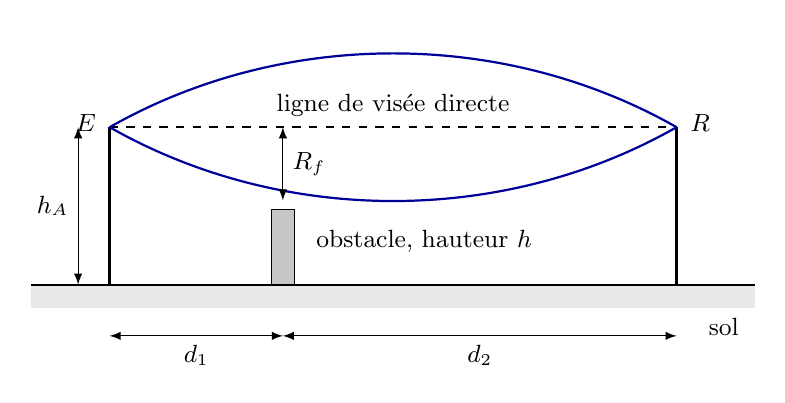
\begin{tikzpicture}[>=latex,scale=1.0]
    \fill[gray!18] (-0.6,-0.3) rectangle (8.6,0);
    \draw[thick] (-0.6,0) -- (8.6,0);
    \node[below] at (8.2,-0.3) {\small sol};
    \draw[very thick] (0.4,0) -- (0.4,2.0);
    \draw[very thick] (7.6,0) -- (7.6,2.0);
    \node[left] at (0.35,2.05) {\small $E$};
    \node[right] at (7.65,2.05) {\small $R$};
    \draw[<->] (0.0,0) -- (0.0,2.0) node[midway,left] {\small $h_A$};
    \draw[thick,dashed] (0.4,2.0) -- (7.6,2.0);
    \node[above] at (4.0,2.02) {\small ligne de visée directe};
    \draw[thick,blue!60!black] (0.4,2.0) .. controls (2.6,3.25) and (5.4,3.25) .. (7.6,2.0);
    \draw[thick,blue!60!black] (0.4,2.0) .. controls (2.6,0.75) and (5.4,0.75) .. (7.6,2.0);
    \draw[<->] (2.6,2.0) -- (2.6,1.07) node[midway,right] {\small $R_f$};
    \draw[fill=gray!45] (2.45,0) rectangle (2.75,0.95);
    \node[right] at (2.9,0.55) {\small obstacle, hauteur $h$};
    \draw[<->] (0.4,-0.65) -- (2.6,-0.65) node[midway,below] {\small $d_1$};
    \draw[<->] (2.6,-0.65) -- (7.6,-0.65) node[midway,below] {\small $d_2$};
  \end{tikzpicture}
\end{figure}

\begin{problem}[Espace dégagé --- ellipsoïde de Fresnel]
  Deux antennes $E$ et $R$, situées à une hauteur $h_A = 20$~m du sol, sont
  séparées d'une distance $d = 10$~km pour lesquelles nous souhaitons établir
  une communication à une fréquence porteuse $f = 2.5$~GHz. On supposera sur
  cette distance que le sol forme un plan.
  \begin{subpart}
    \item Calculer $R_f$ à mi-chemin. Est-ce que la hauteur des antennes est
      suffisante pour que le sol soit en dehors de l'ellipsoïde ?
    \item Un obstacle est situé à $3$~km de l'antenne $E$. Déterminer sa
      hauteur $h$ maximale pour que la liaison soit encore considérée comme
      dégagée.
    \item Dans le cas où il n'y a pas d'obstacle, avec $G_E = G_R = 20$~dB et
      $P_E = 5$~W, calculer la puissance reçue $P_R$.
  \end{subpart}
\end{problem}

\begin{proof}
  À $2.5$~GHz, $\lambda = 12$~cm.\\

  \emph{(a)} Avec $d_1 = d_2 = 5$~km, les dimensions étant en m,
  \[ r = \sqrt{12 \times 10^{-2} \times \frac{25 \times 10^{6}}{10 \times 10^{3}}}
       = \sqrt{300} = 17.3\ \mathrm{m} < h_A = 20\ \mathrm{m}, \]
  donc la hauteur d'antenne est suffisante pour que l'influence du sol sur le
  lien radio soit minimisée. Une hauteur insuffisante occasionnerait des
  phénomènes d'interférences supplémentaires.\\

  \emph{(b)} Avec $d_1 = 3$~km et $d_2 = 7$~km,
  \[ r' = \sqrt{\lambda \frac{d_1 d_2}{d_1+d_2}}
        = \sqrt{12 \times 10^{-2} \times \frac{21 \times 10^{6}}{10^{4}}} = 15.8\ \mathrm{m}, \]
  so the ellipsoid's lower edge is at $h_A - r' = 20 - 15.8 = 4.2$~m. Un
  bâtiment de plus de $4$~m de haut (inférieur à la hauteur d'une maison) sera
  déjà un obstacle non négligeable pour cette liaison malgré un lien en vue
  directe entre les deux antennes.\\

  \emph{(c)} Les gains d'antenne, en échelle linéaire, sont
  $G_E = G_R = 100$ ; $P_E = 5$~W $= 37$~dBm, et
  \[ P_R = P_E G_E G_R \left(\frac{\lambda}{4\pi d}\right)^2
    = 5 \times 100 \times 100 \times \left(\frac{12 \times 10^{-2}}{4\pi \times 10^{4}}\right)^{2}
    \approx 5 \times 10^{-8}\ \mathrm{W}, \]
  ce qui correspond à $-73$~dBW ou $-43$~dBm, which is also read off directly
  as $37 + 20 + 20 - 120$ with $120$~dB of affaiblissement en espace libre.
  \qed
\end{proof}

\subsubsection{Facteurs influençant la propagation}

L'équation de Friis a été obtenue avec l'hypothèse d'une propagation dans le
vide sans obstacles. Or dans la réalité, l'influence de l'environnement sur la
propagation est importante : lors de la propagation, le signal subit de
l'absorption, de la diffraction, des réflexions, de la \textbf{diffusion}
(\textit{scattering}), de la réfraction, etc.

\paragraph{Absorption dans la basse atmosphère} Lors de la propagation d'un
signal dans l'atmosphère, celui-ci subit un affaiblissement linéique (en dB/km)
dû à l'absorption des molécules de dioxygène et des molécules d'eau. Cette
absorption dépend de la fréquence du signal ; on remarque en particulier des
pics d'absorption :

\begin{center}
  \begin{tabular}{@{}ll@{}}
    \toprule
    Molécules & Raies d'absorption \\
    \midrule
    H$_2$O & $22.3$~GHz, $183.3$~GHz, $323$~GHz \\
    O$_2$  & $60$~GHz, $118.74$~GHz \\
    \bottomrule
  \end{tabular}
\end{center}

The reference curve is the affaiblissement linéique par les gaz de
l'atmosphère (ITU-R 719), pression : $1013.6$~mbar, température :
$20\,^\circ$C, vapeur d'eau : $7.5$~g/m$^3$. L'application visée
(communications longue portée ou discrètes) oriente le choix de la fréquence:
the $60$~GHz O$_2$ line is avoided for range and sought, on the contrary, for
deliberately discreet short-range confinement.

\paragraph{Atténuation due à la pluie} La présence de pluie sur une liaison
peut induire une atténuation plus ou moins importante. Two monotonicities hold:
pour une fréquence donnée, plus la pluie est forte, plus l'atténuation est
importante ; pour un taux de pluie donné, l'atténuation augmente avec la
fréquence. Dans les régions tempérées, on considère que la pluie a un effet
significatif au-delà de $5$~GHz, et un effet prépondérant au-delà de $10$~GHz.

\begin{remark}
  L'atténuation due à la pluie se calcule en multipliant l'affaiblissement
  linéique par la \emph{longueur du trajet dans la tranche de pluie}, not by
  the whole link length. It is what fixes the disponibilité de la communication
  en cas de pluie, and therefore the margin that must be carried in the bilan
  de liaison.
\end{remark}

\paragraph{Influence du sol} Le sol est un milieu non magnétique de permittivité
complexe
\[ \bar{\epsilon} = \epsilon - j \frac{\sigma}{\epsilon_0 \omega}. \]
Below a transition frequency the ground behaves as a conducteur, above it as a
diélectrique:
\[ f < f_{\mathrm{transition}} \Rightarrow \text{conducting ground}, \qquad
   f > f_{\mathrm{transition}} \Rightarrow \text{dielectric ground}, \]
avec $f_{\mathrm{transition}} \approx 20$~GHz pour l'eau pure, $\approx 1$~GHz
pour l'eau de mer, et $0.6 - 6$~MHz pour les sols non maritimes. Conséquences
pour un bilan de liaison : prise en compte de l'image de l'antenne (its image
in the ground) ; correction
du facteur de réflexion en fonction de la composition du sol, du relief et de
la distance entre antennes.

\paragraph{Diffraction par le sol} La diffraction par une arête (montagne,
colline) can be computed by treating the obstacle as une arête sans épaisseur.
The practical consequence: sans visibilité directe, on peut tout de même
effectuer une liaison, at the cost of the diffraction loss.

\subsubsection{Milieu réel : modèle de propagation empirique}

Dans le cas d'un environnement complexe (une ville par exemple), où
généralement il n'y a plus de trajet en visibilité directe entre une antenne
d'émission (station de base) et une antenne de réception (smartphone), il est
difficile, voire impossible, de décrire par une relation déterministe
l'atténuation supplémentaire engendrée par le canal de propagation présentant
des trajets multiples (bâtiments, végétation). Pour évaluer l'atténuation dans
ces environnements, la modélisation empirique est utilisée. Les modèles sont
établis à partir de données de mesures d'affaiblissement pour des
environnements types (urbain, suburbain, rural) et utilisables dans de nombreux
cas. Ces modèles permettent aussi bien la planification, en estimant par
simulation l'emplacement optimal d'une station de base dans une cellule, que la
qualification d'un système de communications numériques. De nombreux modèles
d'affaiblissement ont été développés (Hata, Okumura-Hata, 3GPP, Wiener) pour
différents environnements, bandes de fréquence, topographies régionales.

\begin{definition}[Okumura-Hata, rural, $h_m \le 1.5$~m]
  L'influence de la hauteur du mobile étant alors peu significative, le modèle
  d'affaiblissement applicable peut s'écrire
  \begin{align*}
    \mathrm{PL}_{R\text{-}HATA}\,[\mathrm{dB}] =\ & 69.55 + 26.16 \log_{10}(f)
      - 13.82 \log_{10}(h_{bs})
      + \bigl(44.9 - 6.55 \log_{10}(h_{bs})\bigr) \log_{10}(d) \\
      & - 4.78 \left(\log_{10}(f)\right)^{2} + 18.33 \log_{10}(f) - 40.94 .
  \end{align*}
  Les coefficients numériques sont déterminés et tabulés à partir de l'analyse
  des campagnes de mesure effectuées pour chaque type d'environnement.
\end{definition}

\begin{remark}[Units are not SI here]
  Les dimensions des paramètres utilisées dans le modèle de propagation
  Okumura-Hata sont \emph{à conserver telles qu'elles sont} --- the units in
  which the model was fitted: $f$ en MHz, $h_{bs}$ en mètres, $d$ en
  kilomètres. This is the standard trap.
\end{remark}

\begin{problem}[Modèle de propagation empirique]
  Une communication GSM en milieu rural : fréquence $f = 948$~MHz,
  $d = 20$~km, hauteur de la station de base $h_{bs} = 130$~m, hauteur du
  mobile $h_m = 1.5$~m, $G_E = 14$~dB, $G_R = 0$~dB, $P_E = 8$~W. Sur la base
  de la relation
  $P_{R,\mathrm{dBm}} = P_{E,\mathrm{dBm}} + G_{E,\mathrm{dB}} + G_{R,\mathrm{dB}} - L_{\mathrm{dB}}$,
  calculer la puissance $P_R$ disponible au niveau du récepteur du téléphone
  pour le modèle Okumura-Hata et pour le modèle simple de Friis, puis calculer
  la distance $d'$ équivalente avec le modèle de Friis pour la puissance reçue
  obtenue avec le modèle Okumura-Hata.
\end{problem}

\begin{proof}
  Term by term, l'affaiblissement de propagation avec le modèle Okumura-Hata
  rural vaut, avec $f$ en MHz, $h_{bs}$ en m et $d$ en km :
  \[ \mathrm{PL}_{R\text{-}HATA} = 69.55 + 77.87 - 29.2 + 40.36 - 42.35 + 54.56 - 40.94
     \approx 130\ \mathrm{dB}. \]
  Avec $P_E = 8$~W $= 39$~dBm, la puissance reçue vaut
  \[ P_{R,\mathrm{dBm}} = 39 + 14 + 0 - 130 = -77\ \mathrm{dBm}. \]
  Dans le cas de l'application de l'équation de Friis : $\lambda = 0.316$~m,
  $d = 20 \times 10^{3}$~m, et
  \[ \mathrm{PL} = 20 \log_{10}\frac{4 \pi d}{\lambda} = 118\ \mathrm{dB},
     \qquad P_{R,\mathrm{dBm}} = 39 + 14 + 0 - 118 = -65\ \mathrm{dBm}. \]
  Enfin, pour obtenir avec l'équation de Friis le niveau de puissance reçue
  calculé avec le modèle Okumura-Hata,
  \[ 20 \log_{10}\left(\frac{4 \pi d'}{0.316}\right) = 39 + 14 + 77 = 130\ \mathrm{dB}
     \;\Longrightarrow\; d' \approx 78\ \mathrm{km}. \qed \]
\end{proof}

\begin{conclusion}
  The two models disagree by $12$~dB at $20$~km, and translating that gap into
  range turns $20$~km into $78$~km. Ceci indique qu'il est important de faire
  un choix pertinent du modèle d'affaiblissement que l'on utilise pour estimer une
  portée (distance maximale de couverture) lorsque le cahier des charges impose
  un niveau de sensibilité, qui représente la puissance minimale détectable par
  le système de réception pour garantir une qualité de service demandée: that
  level turns directly into a claimed coverage radius, and an optimistic model
  overstates that radius by a factor of four.
\end{conclusion}
